\section{Giới thiệu Grafana}
Theo giới thiệu trên trang chủ của Grafana
"Truy vấn, trực quan hóa, cảnh báo và hiểu dữ liệu của bạn không quan trọng nó được lưu trữ ở đâu. Với Grafana bạn có thể tạo, khai phá, chia sẻ dữ liệu của mình thông qua những dashboard đẹp và linh động"
\begin{figure}[H] % places figure environment here   
    \centering % Centers Graphic
    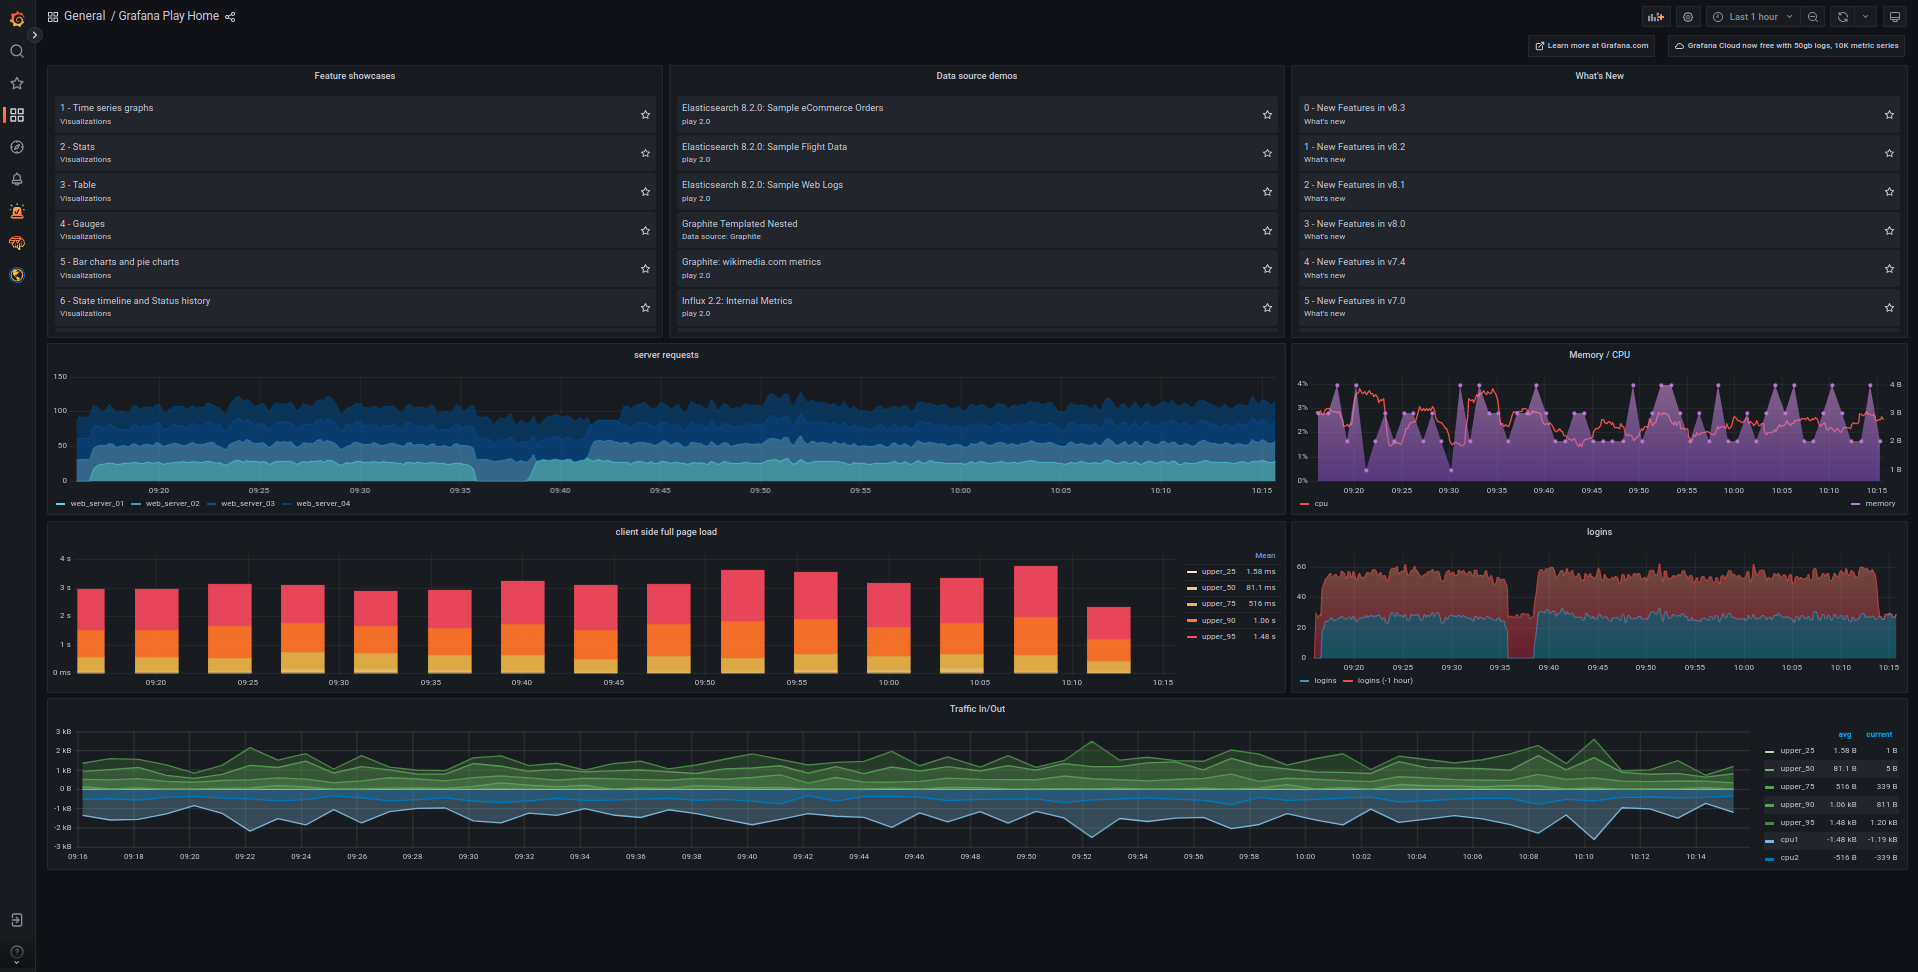
\includegraphics[width=1\textwidth]{figures/fig_01.png} 
    \caption{Một dashboard demo trên trang chủ của Grafana} % Creates caption underneath graph
    \label{fig:fig_01}
\end{figure}
Biểu đồ trên cùng bên trái thể hiện lượng requests tới một website nào đó trong khoảng thời gian một giờ gần nhất. Không chỉ thể hiện tổng lượng request, ta còn có thể quan sát thấy thông lượng tới từng node từ web\_server\_01 đến web\_server\_04 thông qua lớp phủ màu. Ngoài ra khi giữ chuột vào một thời điểm nhất định, biểu đồ cũng cho biết số lượng request cụ thể vào từng node vào thời điểm đó. 

Biểu đồ trên cùng bên phải thể hiện tài nguyên Memory và CPU được sử dụng của ứng dụng. 
